\subsection{Energy efficiency}

To save energy, the following techniques and features are used.

\subsubsection{Low energy modes}

\begin{figure}[H]
\centering
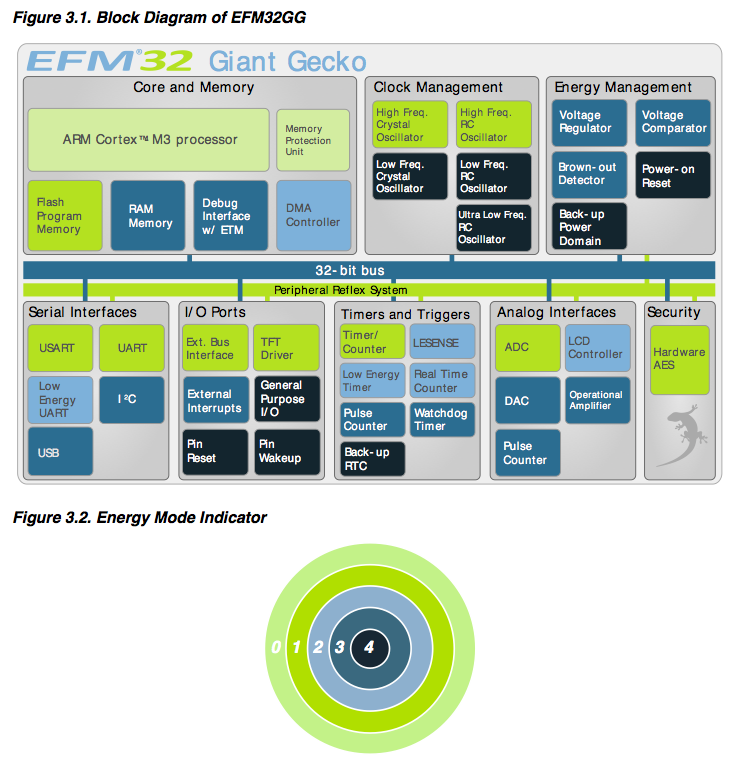
\includegraphics[width=0.75\textwidth]{figures/energymodes.png}
\caption{The energy modes of the Giant Gecko Micro Controller}
\label{fig:energymodes}
\end{figure}

The Giant Gecko micro controller has four different energy modes, with different peripherals available in each mode.

Whenever possible, the micro controller should enter a sleep mode to conserve energy.
In this implementation, the micro controller enters energy mode 2 when none of the timers are running, and energy mode 1 when playing a song or checking the buttons.

The only time the program needs to enter energy mode 0, is when the state machine needs updating.
This consumes a lot of power, but is considered a choice.
In a very simple application such as this, where all events that require an FSM update are generated by a single timer, the FSM can be updated from this interrupt service routine.
However in a more realistic application, events would be generated by several different sources, and updating the FSM in all of these different places is not desirable.

\subsubsection{Turning off unused GPIO}
When the micro controller is doing other things, having GPIO lines enabled can cause so called GPIO leakage.
This might lead to extra power usage.
To prevent this, all unused GPIO ports are turned off.

\subsubsection{Disabling timers whenever possible}
Any timer will use more power while it is active, so it is not good practice to leave them on.
To save power, the button debounce timer is enabled in response to a GPIO interrupt, and the song timer is enbabled in response to a play event. 

\subsubsection{Using DAC in sample and hold mode}
The DAC is configured in Sample/Hold Mode, which means that the DAC core is turned off between sample conversions.
The DAC core converts data on triggered conversion and holds the the output in a sample/hold element.
This element will only be held for a certain period of time because of output voltage drift.
The sampling period is set to the length of one prescaled clock cycle.

\subsubsection{Further work}
There could be done a few more energy saving measures, but due to taking to much work, they were not implemented.


\begin{description}
  \item[Use low energy timer (LETIMER) for checking buttons.] \hfill \\
        In the current implementation, a normal timer is used for input detection. This is not necessary, as a low energy timer would be sufficient. 
  \item[Use DMA to push samples to the DAC] \hfill \\
        With Direct Memory Access, it would be possible to stay in low energy mode when loading music to the DAC, saving a lot of energy.
\end{description}



